%=====================================================================
\section{Station capacity (E9): guns per station and power per gun}
\label{sec:e9}

Station capacity is the second of the three factors the course asks the analysis to study (the first, the number of mobile chargers, is E2, covered earlier in this Part). A fixed charging station (FCS) has two capacity knobs:
\begin{itemize}
  \item \textbf{guns} (charging points) per station: how many cars a station can charge \emph{at the same time};
  \item \textbf{power} per gun (kW): how \emph{fast} each car charges.
\end{itemize}
The baseline has 2 guns of 22\,kW at each station. Experiment E9 halves and doubles each knob on its own: 1 or 4 guns, 11 or 44\,kW. Every variant is solved by reinforcement learning with a model \emph{retrained} for that setting (there is no MILP for E9/E10; the RL policy, shown throughout this report to track the MILP closely, is used as the fast, faithful tool). The four variants are measured against the baseline RL plan on the instances where both are feasible.

\begin{figure}[H]
\centering
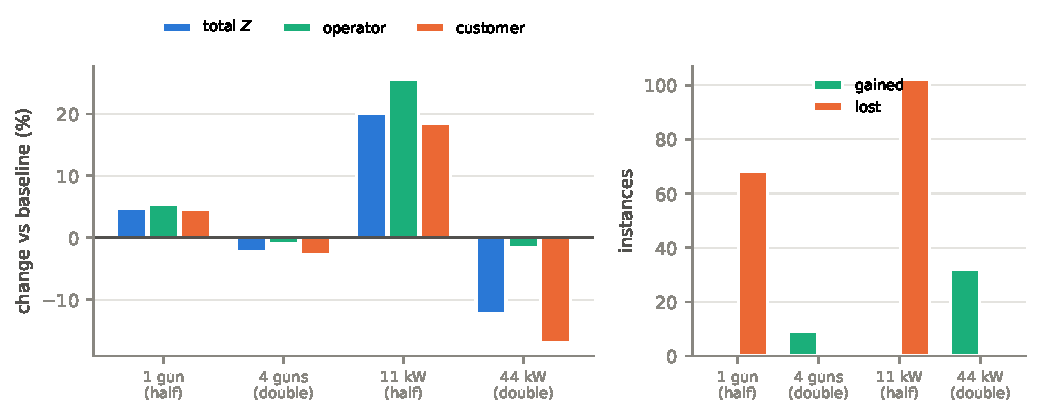
\includegraphics[width=\textwidth]{figures/exp_e9.pdf}
\caption{E9 station capacity. Left: change of the total cost $Z$ and of its operator and customer parts against the baseline (\%, paired instances). Right: instances that gain or lose a feasible plan.}
\label{fig:e9}
\end{figure}

\begin{table}[H]
\centering
\caption{E9, retrained RL. ``comm.\ queue'' and ``van \% pers.'' are shown baseline $\to$ variant. ``gained''/``lost'': instances that become feasible / infeasible. ``paired'': instances feasible in both.}
\scriptsize
\begin{adjustbox}{max width=\linewidth}
\begin{tabular}{@{}llrrrllrrr@{}}
\toprule
variant & what changes & \shortstack{$\Delta Z$\\\%} & \shortstack{$\Delta$\\oper. \%} & \shortstack{$\Delta$\\cust. \%} & \shortstack{comm. queue\\(min)} & van \% pers. & gained & lost & paired \\
\midrule
E9\_guns\_1 & 1 gun per station (half) & $+$4.76 & $+$5.40 & $+$4.55 & 1.18 $\to$ 3.48 & 6.2 $\to$ 16.7 & 0 & 68 & 432 \\
E9\_guns\_4 & 4 guns per station (double) & $-$2.21 & $-$0.90 & $-$2.72 & 2.50 $\to$ 0.53 & 6.7 $\to$ 5.3 & 9 & 0 & 500 \\
E9\_power\_11 & 11 kW per gun (half) & $+$20.13 & $+$25.61 & $+$18.43 & 1.25 $\to$ 0.77 & 6.3 $\to$ 58.7 & 0 & 102 & 398 \\
E9\_power\_44 & 44 kW per gun (double) & $-$12.30 & $-$1.54 & $-$16.97 & 2.50 $\to$ 2.32 & 6.7 $\to$ 0.0 & 32 & 0 & 500 \\
\bottomrule
\end{tabular}
\end{adjustbox}

\end{table}

\subsection{What the numbers say}
\begin{itemize}
  \item \textbf{Power is the strong lever, guns the weak one.} Halving the power to 11\,kW changes $Z$ by \feNinePowHalfDz\,\%; doubling it to 44\,kW by $-$\feNinePowDblDzAbs\,\%. Halving or doubling the \emph{guns} moves $Z$ only by \feNineGunsHalfDz\,\% and $-$\feNineGunsDblDzAbs\,\%.
  \item \textbf{The two knobs act through different channels.} Fewer guns triple the commercial queue (\feNineGunsHalfQBase{} $\to$ \feNineGunsHalfQ{} min): with one gun the cars at a station must wait their turn. Lower power barely changes the queue; instead it makes station charging so slow that charging moves onto the vans --- the personal van share jumps from about 6\,\% to \feNinePowHalfVan\,\%.
  \item \textbf{Capacity decides feasibility.} Weaker capacity strands cars that can no longer be charged before the deadline: \feNinePowHalfLost{} instances lose a feasible plan at 11\,kW and \feNineGunsHalfLost{} at 1~gun. Stronger capacity rescues some: \feNinePowDblGain{} at 44\,kW, \feNineGunsDblGain{} at 4~guns.
\end{itemize}

\inshort{Power per gun is the dominant capacity lever (about $\pm$12--20\,\% on $Z$); the number of guns matters much less (about $\pm$2--5\,\%) and only through queueing. Cutting capacity also strands dozens of instances.}

\subsection{Why: the charging-time law}

\begin{figure}[H]
\centering
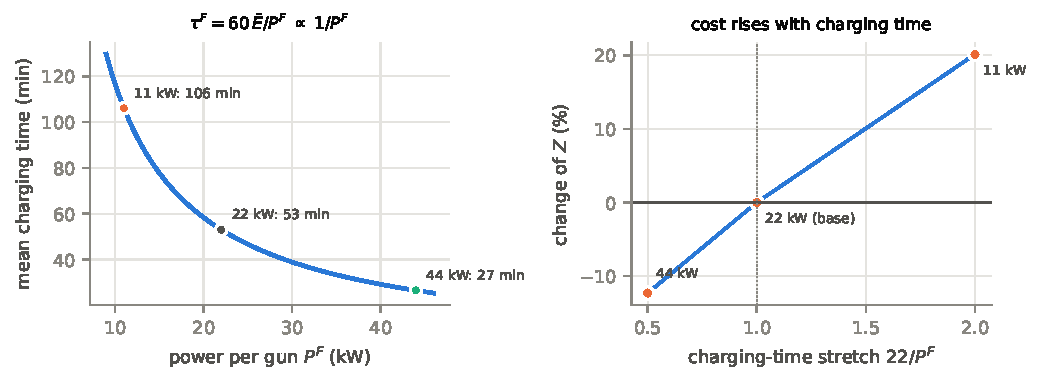
\includegraphics[width=\textwidth]{figures/exp_e9_power.pdf}
\caption{Left: FCS charging time against power per gun --- an inverse law. Right: the measured change of $Z$ rises with the charging-time ``stretch'' $22/P^F$.}
\label{fig:e9power}
\end{figure}

The whole pattern follows from one identity in the model.

\begin{keybox}
\textbf{Proposition 1 (charging-time law).} The time an EV $i$ spends charging at an FCS is
\[
\tau^F_i \;=\; \frac{60\,E_i}{P^F}\quad\text{minutes},
\]
where $E_i$ is its energy demand (kWh) and $P^F$ the power per gun (kW). Hence $\tau^F_i \propto 1/P^F$: scaling the power by a factor $\rho$ scales \emph{every} FCS charging time by $1/\rho$.\\[2pt]
\textbf{Proof.} Energy $=$ power $\times$ time, so the charging time in hours is $E_i/P^F$; $\times 60$ gives minutes. The power $P^F$ appears only in the denominator, so $\tau^F_i$ is inversely proportional to it. $\square$
\end{keybox}

With the mean demand $\bar E \approx \fmeanEnergy$\,kWh, the baseline charging time is $\tau^F=\feNineTauBase$\,min; halving the power doubles it to \feNineTauHalf\,min, doubling it halves it to \feNineTauDbl\,min (Figure~\ref{fig:e9power}, left). Power changes the \emph{time} a car charges, not the \emph{energy} it draws, so the operator's electricity bill ($Z_4$) is untouched; what moves is every time-cost term that contains $\tau^F$.

\begin{keybox}
\textbf{Proposition 2 (power is first order, guns are second order).} Write the customers' charging-time cost as $Z_{\text{chg}}=\sum_i c^C_i\,\tau^F_i=\dfrac{60}{P^F}\sum_i c^C_i E_i$, a part of $Z_6$. Then $Z_{\text{chg}}\propto 1/P^F$, so power acts on this large term directly. The number of guns does \emph{not} enter $\tau^F_i$; it only sets how many cars may charge in parallel at a station (the gun-load constraint), and so changes $Z$ only through the queue term $\sum_i c^Q_i\,\tau^Q_i$. Because the mean queue ($\approx$1--2\,min) is far smaller than the mean charging time ($\feNineTauBase$\,min), $\bigl|\partial Z/\partial(\text{power})\bigr|\gg\bigl|\partial Z/\partial(\text{guns})\bigr|$.\\[2pt]
\textbf{Proof.} $P^F$ enters the objective only through $\tau^F_i=60E_i/P^F$ in the charging-time terms, giving the stated $1/P^F$ law. The gun count enters only the per-station capacity constraint (at most ``guns'' cars charging at once), which bounds the queueing delay $\tau^Q_i$ but leaves $\tau^F_i$, $E_i$ and the tariff unchanged. The size of each lever is the size of the term it scales; charging time dominates queueing time in the data by more than an order of magnitude. $\square$
\end{keybox}

This is exactly what the experiment shows: power moves $Z$ by $\pm$12--20\,\%, guns by $\pm$2--5\,\%, and the guns variants move the \emph{queue} while the power variants move the \emph{van share}.

\textbf{Why the van share explodes at low power.} When the FCS takes \feNineTauHalf\,minutes, station charging becomes so slow that a van --- which charges a car wherever it stands, with no station queue and no driver waiting --- becomes worth its premium even for private owners who would normally use a station. The policy therefore sends \feNinePowHalfVan\,\% of free-choice personal cars to vans (against about 6\,\% at the baseline). At 44\,kW the station is so fast (\feNineTauDbl\,min) that the van's advantage disappears and the personal van share falls to~0. The van is the model's release valve for expensive station time: the clearest possible sign that FCS charging time is the binding cost.

\begin{keybox}
\textbf{Proposition 3 (the effect is asymmetric, by convexity).} Under power $P^F\!\to\!\rho P^F$ the charging time changes by $\Delta\tau=\tau^F(1/\rho-1)$. Because $\tau^F(P)\propto 1/P$ is convex, halving the power ($\rho=\tfrac12$) \emph{adds} $\tau^F$ minutes ($+\feNineTauBase$) while doubling it ($\rho=2$) \emph{removes} only $\tau^F/2$ ($-\!\approx\!27$). Hence the cost rise from halving exceeds the cost fall from doubling, as observed ($+\feNinePowHalfDz$\,\% vs $-$\feNinePowDblDzAbs\,\%).\\[2pt]
\textbf{Proof.} $\tau^F(\rho P)=\tau^F(P)/\rho$, so $\Delta\tau(\rho=\tfrac12)=\tau^F$ and $\Delta\tau(\rho=2)=-\tau^F/2$; $|\!+\!\tau^F|>|\!-\!\tau^F/2|$. The cost terms are increasing in $\tau^F$, so their change inherits this inequality. The asymmetry is reinforced by the deadline $C_i\le T$: at half power the completion time binds for many cars (\feNinePowHalfLost{} become infeasible and the survivors pay heavily), whereas at double power the deadline is already slack, so the extra speed has no value once a car is charged in time --- the benefit saturates. $\square$
\end{keybox}

\inshort{One identity, $\tau^F=60E/P^F$, explains E9. Power scales the dominant charging-time cost as $1/P^F$ (a convex, hence asymmetric, law) and, when low enough, pushes charging onto vans; guns touch only the small queue term. Below a point, cutting capacity makes instances infeasible rather than merely dearer.}
